\documentclass[border=3pt]{standalone}
% Preâmbulo compartilhado pelos diagramas TikZ da aula 8 de IHC (Design de IHC)
\usepackage[T1]{fontenc}
\usepackage[utf8]{inputenc}
\usepackage{lmodern}
\usepackage{amsmath}
\usepackage{xcolor}
\usepackage{tikz}
\usetikzlibrary{arrows.meta,angles,quotes,decorations.pathmorphing,decorations.pathreplacing,calc,
                positioning,shapes.geometric,shapes.misc,backgrounds,fit,
                math}

% Paleta (mesma dos SVGs originais)
% Paleta da disciplina de IHC: acento roxo (#755099), da capa do livro.
% (o nome "dblue" é mantido para não alterar todos os diagramas)
\definecolor{dblue}{HTML}{755099}
\definecolor{dorange}{HTML}{B3541E}
\definecolor{dgreen}{HTML}{4A7C59}
\definecolor{dred}{HTML}{9C4B4B}
\definecolor{dcream}{HTML}{F4F1EA}
\definecolor{dshade}{HTML}{DDD7C9}

% Função gaussiana (não normalizada por padrão de escala visual)
\pgfmathdeclarefunction{gauss}{3}{%
  \pgfmathparse{1/(#3*sqrt(2*pi))*exp(-((#1-#2)^2)/(2*#3^2))}%
}

% Estilos comuns (prefixo d... para não colidir com chaves internas do pgf)
\tikzset{
  >={Stealth[length=2mm]},
  dguide/.style={gray!55, dashed, line width=0.4pt},
  daxis/.style={gray!60, line width=0.7pt, ->},
  dbody/.style={fill=black!3, draw=black!80, line width=1pt},
  dacc/.style={draw=dblue, line width=1pt},
  dlbl/.style={black!55, font=\small},
  dsub/.style={black!45, font=\footnotesize},
  dstate/.style={circle, draw=black!80, fill=dcream, line width=1pt,
                 minimum size=17mm, font=\large, inner sep=1pt},
  dobs/.style={circle, draw=black!80, fill=dshade, line width=1pt,
               minimum size=14mm, font=\large, inner sep=1pt},
  dbox/.style={rounded corners=2pt, draw=black!80, fill=dcream, line width=1pt,
               align=center, inner sep=6pt},
  dop/.style={circle, draw=black!80, fill=white, line width=1pt,
              minimum size=6mm, inner sep=0pt, font=\small},
  dtrans/.style={->, dblue, line width=1pt},
  dmeas/.style={->, dorange, line width=1pt},
  dcurve/.style={line width=1pt, dblue},
  dcurveb/.style={line width=1.4pt, dorange},
}

\begin{document}
\hyphenpenalty=10000 \exhyphenpenalty=10000 \tolerance=9999 \emergencystretch=3em
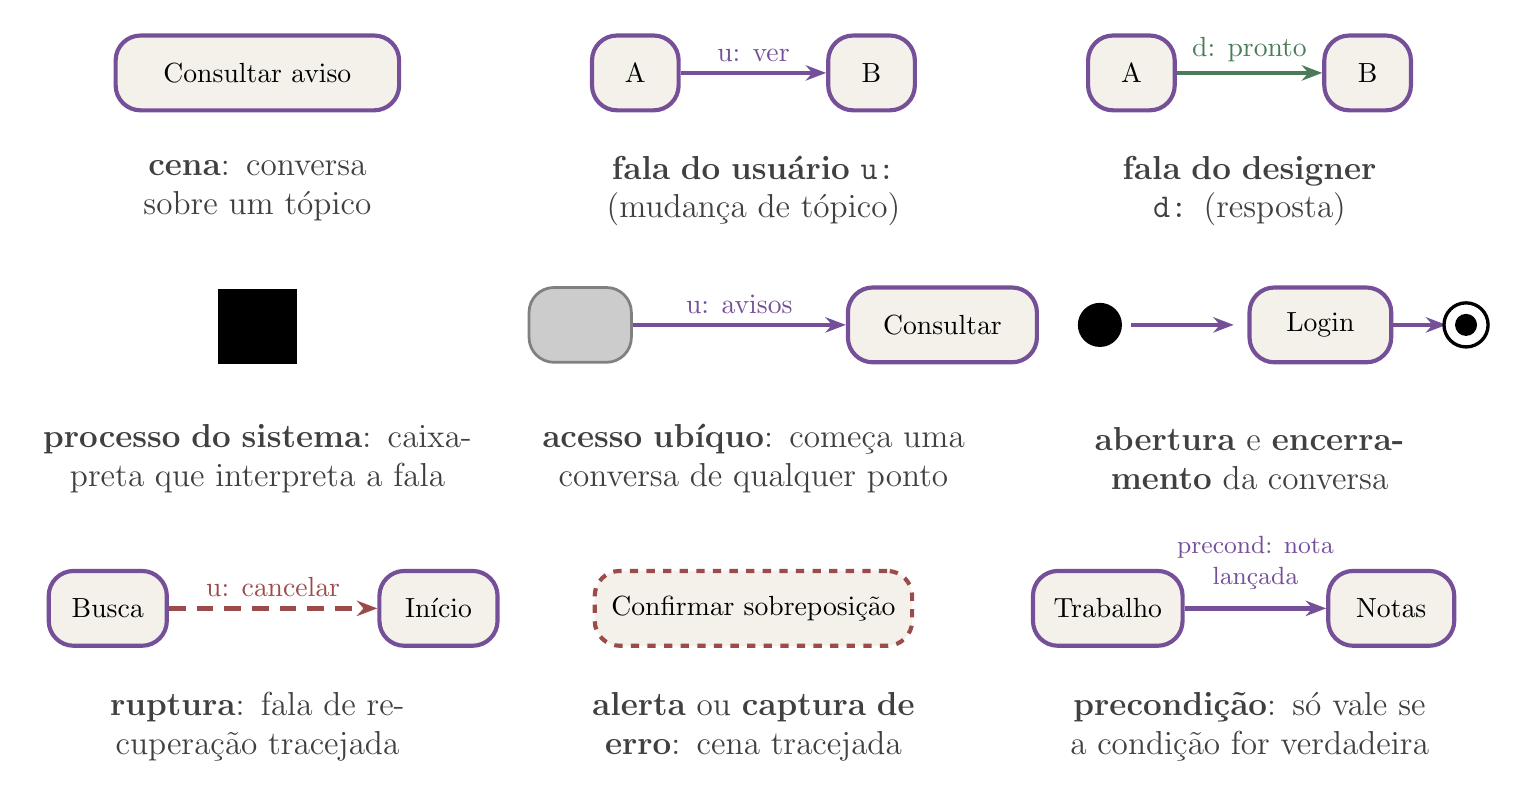
\begin{tikzpicture}[x=1cm,y=1cm]
\node[dbox, draw=dblue, rounded corners=9pt, line width=1.5pt, minimum width=3.6cm, minimum height=0.95cm, font=\normalsize, inner sep=3pt] (a1) at (3.2,7.6) {Consultar aviso};
\node[font=\large, black!75, text width=5.6cm, align=center] at (3.2,6.1) {\textbf{cena}: conversa sobre um tópico};
\node[dbox, draw=dblue, rounded corners=9pt, line width=1.5pt, minimum width=1.1cm, minimum height=0.95cm, font=\normalsize, inner sep=3pt] (b1) at (8.0,7.6) {A};\node[dbox, draw=dblue, rounded corners=9pt, line width=1.5pt, minimum width=1.1cm, minimum height=0.95cm, font=\normalsize, inner sep=3pt] (b2) at (11.0,7.6) {B};\draw[dtrans, line width=1.6pt, -{Stealth[length=2.6mm]}] (b1.east) -- node[above, font=\normalsize] {u: ver} (b2.west);
\node[font=\large, black!75, text width=5.6cm, align=center] at (9.5,6.1) {\textbf{fala do usuário} \texttt{u:} (mudança de tópico)};
\node[dbox, draw=dblue, rounded corners=9pt, line width=1.5pt, minimum width=1.1cm, minimum height=0.95cm, font=\normalsize, inner sep=3pt] (c1) at (14.3,7.6) {A};\node[dbox, draw=dblue, rounded corners=9pt, line width=1.5pt, minimum width=1.1cm, minimum height=0.95cm, font=\normalsize, inner sep=3pt] (c2) at (17.3,7.6) {B};\draw[dgreen, line width=1.6pt, -{Stealth[length=2.6mm]}] (c1.east) -- node[above, font=\normalsize] {d: pronto} (c2.west);
\node[font=\large, black!75, text width=5.6cm, align=center] at (15.8,6.1) {\textbf{fala do designer} \texttt{d:} (resposta)};
\fill[black] (2.7,3.9) rectangle ++(1.0,0.95);
\node[font=\large, black!75, text width=5.6cm, align=center] at (3.2,2.7) {\textbf{processo do sistema}: caixa-preta que interpreta a fala};
\node[dbox, draw=black!50, fill=black!20, rounded corners=9pt, minimum width=1.3cm, minimum height=0.95cm] (u1) at (7.3,4.4) {};\node[dbox, draw=dblue, rounded corners=9pt, line width=1.5pt, minimum width=2.4cm, minimum height=0.95cm, font=\normalsize, inner sep=3pt] (u2) at (11.9,4.4) {Consultar};\draw[dtrans, line width=1.6pt, -{Stealth[length=2.6mm]}] (u1.east) -- node[above, font=\normalsize] {u: avisos} (u2.west);
\node[font=\large, black!75, text width=5.6cm, align=center] at (9.5,2.7) {\textbf{acesso ubíquo}: começa uma conversa de qualquer ponto};
\fill[black] (13.9,4.4) circle (0.28); \draw[dtrans, line width=1.6pt, -{Stealth[length=2.6mm]}] (14.3,4.4) -- (15.6,4.4);\node[dbox, draw=dblue, rounded corners=9pt, line width=1.5pt, minimum width=1.8cm, minimum height=0.95cm, font=\normalsize, inner sep=3pt] (v1) at (16.7,4.4) {Login};\draw[dtrans, line width=1.6pt, -{Stealth[length=2.6mm]}] (17.6,4.4) -- (18.3,4.4); \draw[black, fill=white, line width=1.2pt] (18.55,4.4) circle (0.28); \fill[black] (18.55,4.4) circle (0.14);
\node[font=\large, black!75, text width=5.6cm, align=center] at (15.8,2.7) {\textbf{abertura} e \textbf{encerramento} da conversa};
\node[dbox, draw=dblue, rounded corners=9pt, line width=1.5pt, minimum width=1.5cm, minimum height=0.95cm, font=\normalsize, inner sep=3pt] (r1) at (1.3,0.8) {Busca};\node[dbox, draw=dblue, rounded corners=9pt, line width=1.5pt, minimum width=1.5cm, minimum height=0.95cm, font=\normalsize, inner sep=3pt] (r2) at (5.5,0.8) {Início};\draw[dred, dash pattern=on 6pt off 4pt, line width=1.6pt, -{Stealth[length=2.6mm]}] (r1.east) -- node[above, font=\normalsize] {u: cancelar} (r2.west);
\node[font=\large, black!75, text width=5.6cm, align=center] at (3.2,-0.7) {\textbf{ruptura}: fala de recuperação tracejada};
\node[dbox, draw=dred, dashed, rounded corners=9pt, line width=1.5pt, minimum width=3.8cm, minimum height=0.95cm, font=\normalsize] at (9.5,0.8) {Confirmar sobreposição};
\node[font=\large, black!75, text width=5.6cm, align=center] at (9.5,-0.7) {\textbf{alerta} ou \textbf{captura de erro}: cena tracejada};
\node[dbox, draw=dblue, rounded corners=9pt, line width=1.5pt, minimum width=1.9cm, minimum height=0.95cm, font=\normalsize, inner sep=3pt] (p1) at (14.0,0.8) {Trabalho};\node[dbox, draw=dblue, rounded corners=9pt, line width=1.5pt, minimum width=1.6cm, minimum height=0.95cm, font=\normalsize, inner sep=3pt] (p2) at (17.6,0.8) {Notas};\draw[dtrans, line width=1.6pt, -{Stealth[length=2.6mm]}] (p1.east) -- node[above, font=\small, align=center, yshift=3pt] {precond: nota\\ lançada} (p2.west);
\node[font=\large, black!75, text width=5.6cm, align=center] at (15.8,-0.7) {\textbf{precondição}: só vale se a condição for verdadeira};
\end{tikzpicture}
\end{document}
